\noindent
\textit{\textbf{Regression Discontinuity Results for Different Bandwidths and Functional Forms}} --- 
\afterpage{
    \begin{table}[t!]
        \centering
        \caption{Robustness Checks: For Different Bandwidths}
        \label{Table:Robustness-Checks_BWs}
        \vspace{0.3cm}
        \footnotesize
        \begin{adjustbox}{scale = 0.85}
            \begin{threeparttable}
                \begin{tabular}{@{\extracolsep{5pt}}lcccccccc}
                    \\[-5.5ex]
                    \hline \hline
                    \\[-3.0ex]
                     & \multicolumn{8}{c}{Dependent Variable} \\
                    \\[-3.0ex]
                    \cline{2-9}
                    \\[-3.0ex]
                     & \multicolumn{8}{c}{Average Daily Electricity Consumption  (kWh/Day)} \\
                    \\[-3.0ex]
                     & (1) & (2) & (3) & (4) & (5) & (6) & (7) & (8) \\
                    \\[-3.0ex]
                    \hline
                    \\[-2.0ex]
                    $\mathbb{1}$[Treatment] & $-$0.026 & $-$0.038$^{**}$ & $-$0.039$^{**}$ & $-$0.064$^{***}$ & $-$0.060$^{***}$ & $-$0.061$^{***}$ & $-$0.060$^{***}$ & $-$0.069$^{***}$ \\ 
                    & (0.027) & (0.018) & (0.017) & (0.015) & (0.014) & (0.012) & (0.020) & (0.023) \\ 
                    & & & & & & & & \\ 
                    NC0 & 0.207$^{***}$ & 0.222$^{***}$ & 0.224$^{***}$ & 0.225$^{***}$ & 0.225$^{***}$ & 0.221$^{***}$ & 0.236$^{***}$ & 0.229$^{***}$ \\ 
                    & (0.009) & (0.005) & (0.005) & (0.005) & (0.005) & (0.006) & (0.008) & (0.009) \\ 
                    & & & & & & & & \\ 
                    $\mathbb{1}$[Treatment] $\times$ NC0 & 0.017$^{*}$ & $-$0.006 & $-$0.010$^{***}$ & $-$0.009$^{***}$ & $-$0.009$^{***}$ & $-$0.015$^{***}$ & $-$0.019$^{***}$ & $-$0.017$^{***}$ \\ 
                    & (0.010) & (0.004) & (0.002) & (0.002) & (0.002) & (0.002) & (0.003) & (0.004) \\ 
                    & & & & & & & & \\ 
                    Average Daily CDDs & 1.146$^{***}$ & 1.146$^{***}$ & 1.146$^{***}$ & 1.146$^{***}$ & 1.145$^{***}$ & 1.135$^{***}$ & 1.102$^{***}$ & 1.133$^{***}$ \\ 
                    & (0.105) & (0.106) & (0.106) & (0.105) & (0.105) & (0.109) & (0.115) & (0.129) \\ 
                    & & & & & & & & \\ 
                    Average Daily HDDs & 0.427$^{***}$ & 0.428$^{***}$ & 0.429$^{***}$ & 0.431$^{***}$ & 0.433$^{***}$ & 0.375$^{***}$ & 0.691$^{***}$ & 0.742$^{***}$ \\ 
                    & (0.108) & (0.106) & (0.105) & (0.104) & (0.103) & (0.128) & (0.128) & (0.202) \\ 
                    & & & & & & & & \\
                    \hline
                    \\[-2.0ex]
                    Bandwidth & 5\% & 10\% & 15\% & 20\% & 25\% & 30\% & 35\% & 40\% \\ 
                    FEs: Billing Year-by-Month & Yes & Yes & Yes & Yes & Yes & Yes & Yes & Yes \\ 
                    Observations & 1,186,630 & 2,378,864 & 3,566,318 & 4,702,081 & 5,816,854 & 6,276,579 & 4,093,259 & 3,904,120 \\ 
                    Adjusted R$^{2}$ & 0.282 & 0.293 & 0.311 & 0.334 & 0.361 & 0.536 & 0.550 & 0.592 \\
                    \\[-2.0ex]
                    \hline \hline
                    \\[-4.5ex]
                \end{tabular}
                \begin{tablenotes}[flushleft]
                    \footnotesize
                    \item \textit{Note}: * $p < 0.1$, ** $p < 0.05$, and *** $p < 0.01$.
                \end{tablenotes}
            \end{threeparttable}
        \end{adjustbox}
    \end{table}
}

Table \ref{Table:Robustness-Checks_BWs} summarizes the regression results for a set of different bandwidths. The estimated treatment effect for the households in a very narrow range from the lower base usage quantity (i.e., the households within the bandwidth of 5\%) is not statistically significant even at the 10\% level. Except for the bandwidth of 5\%, the treatment estimates range from $-$0.038 to $-$0.069 and statistically differ from zero at least at the 5\% level. The estimated treatment effect is almost identical for the bandwidths of 10\% and 15\%. For wider bandwidths falling between 20\% and 40\%, the magnitude of the estimated treatment effect increases and remains stable.\footnote{The number of observations increases with the size of the bandwidth exploited, except the two widest ones. The exceptions are because I drop observations crossing the higher base usage quantity to avoid picking up the effect of surpassing the higher cutoff point.} Interestingly, this table clearly shows that the wider the bandwidth employed, the larger the estimated treatment effect. In other words, the treatment estimates approach zero as I move even closer to the lower base usage quantity.

\afterpage{
    \begin{figure}[t!]
        \centering
        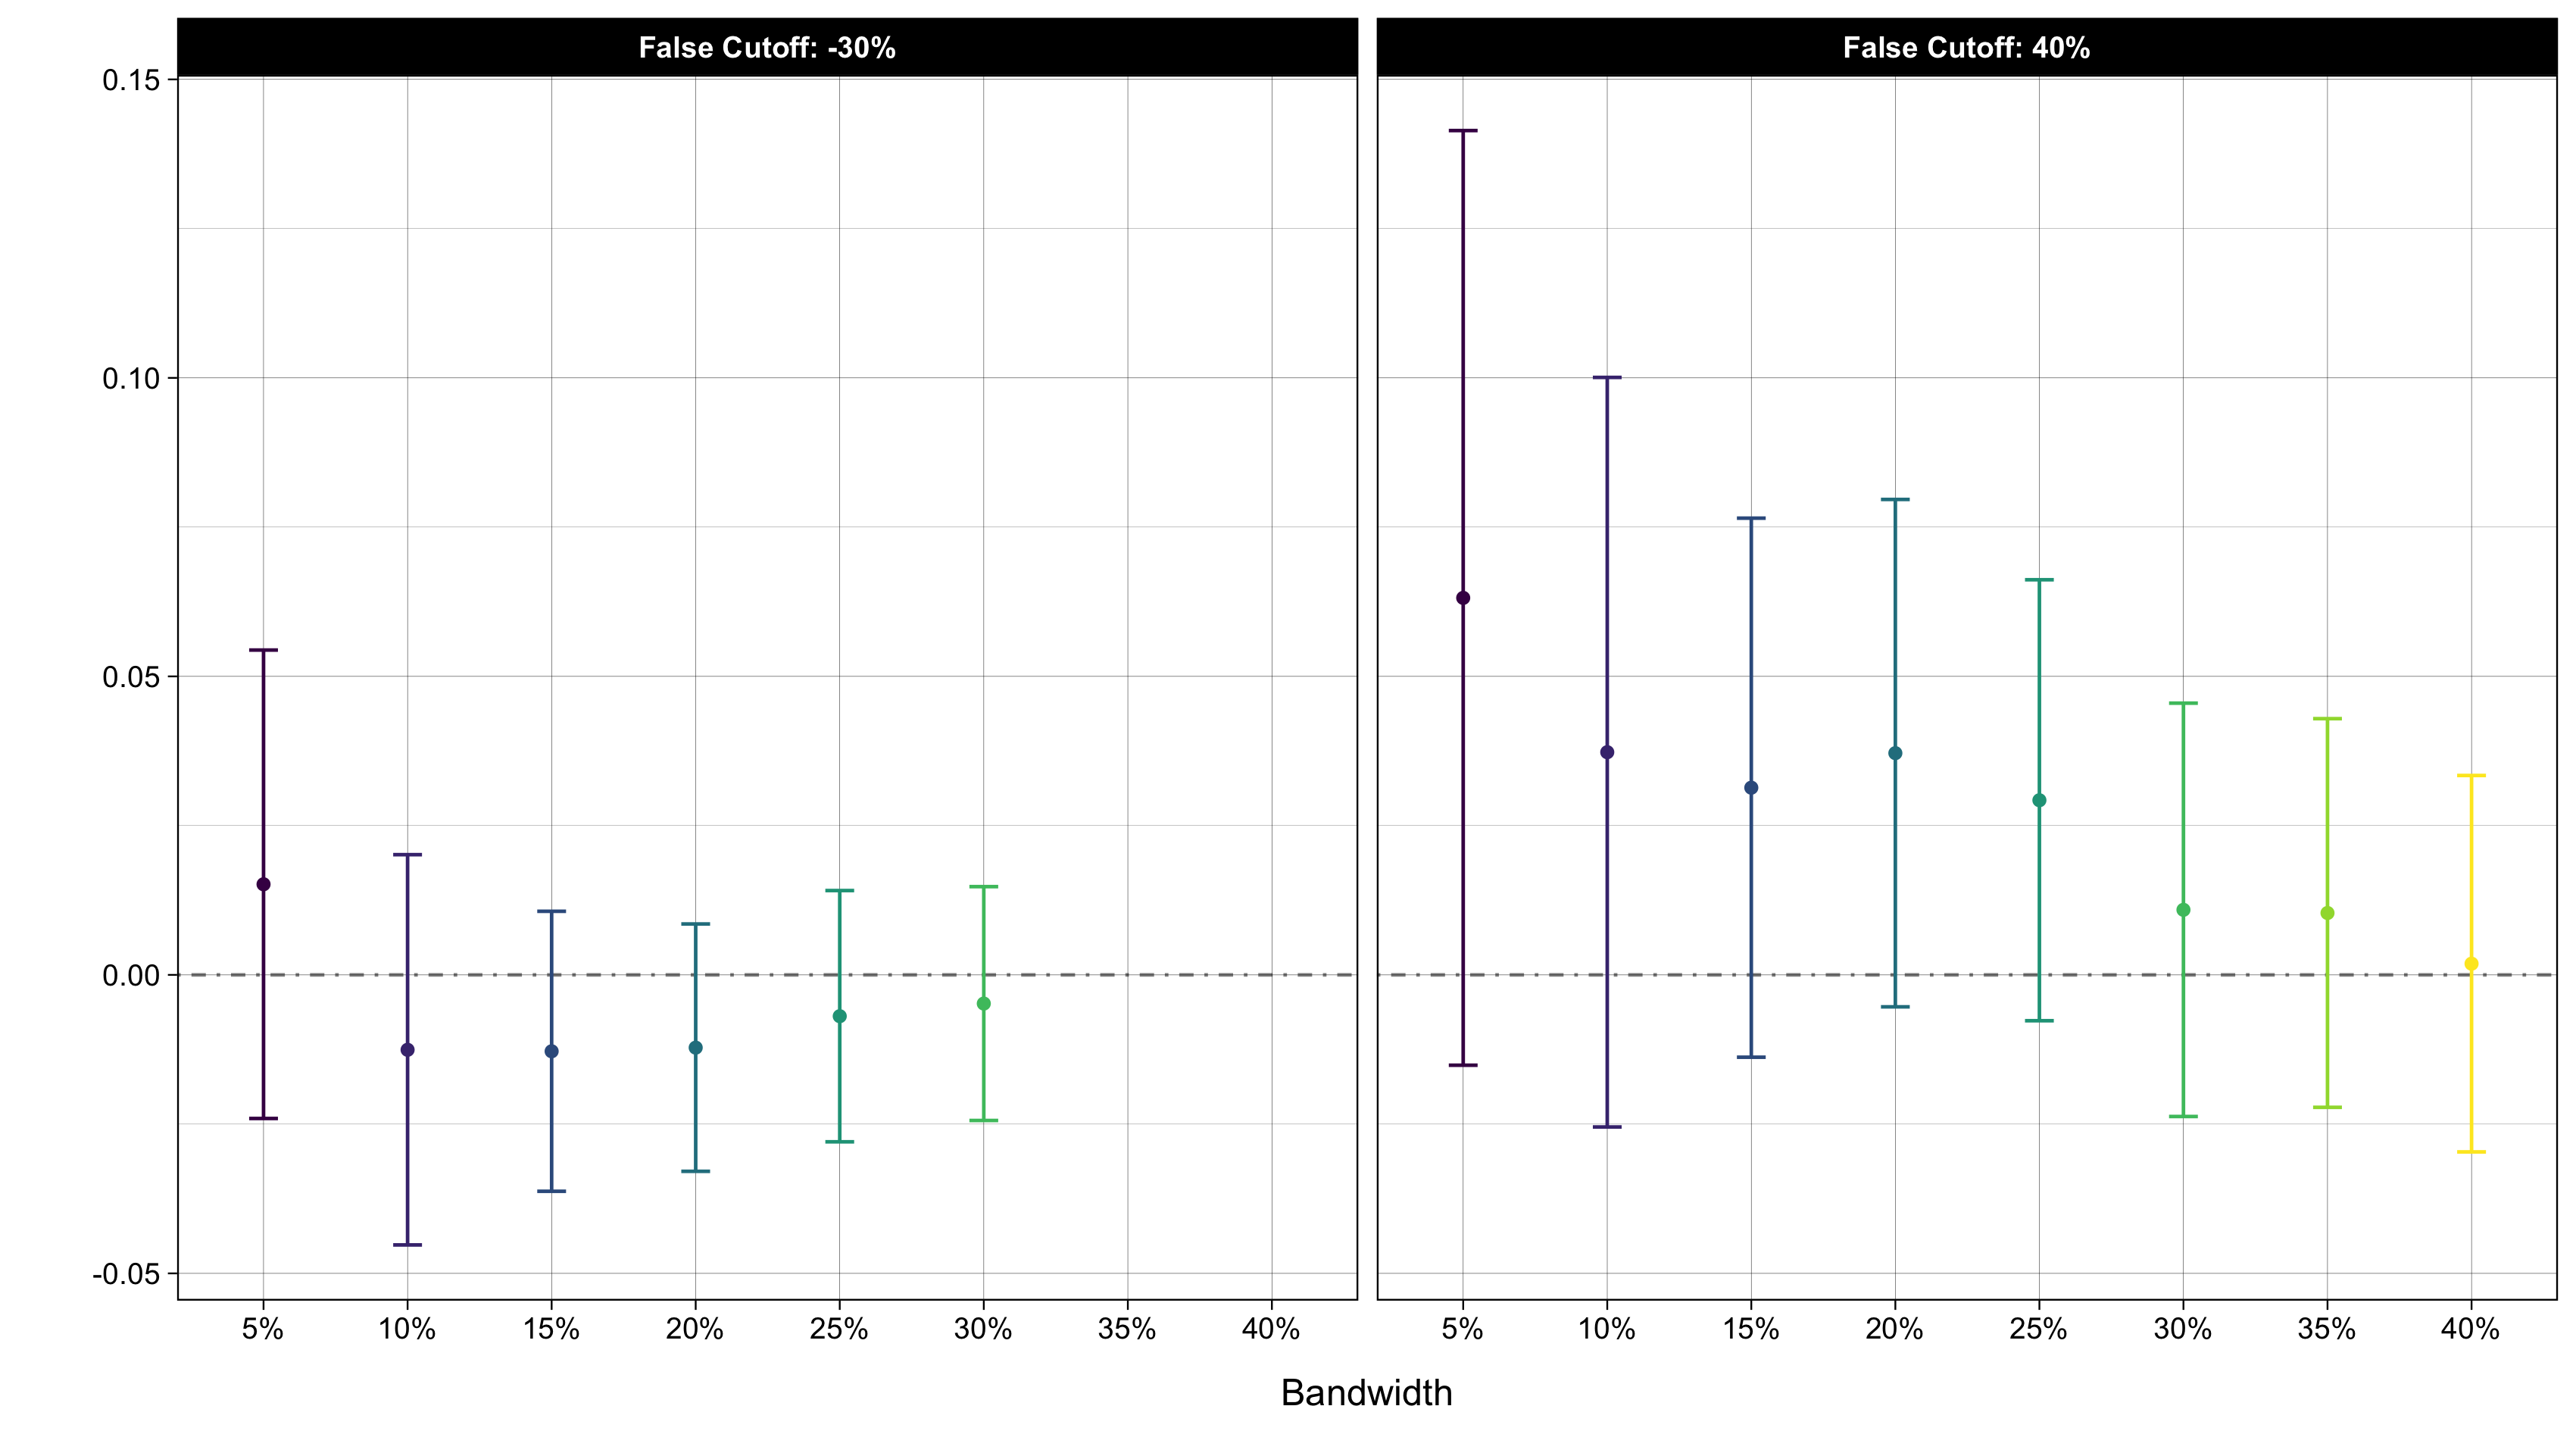
\includegraphics[scale = 0.133]{02_Chapter-1/00A_Figures/Figure_Falsification-Tests_With-False-Cutoff-40-and-M30.png}
        \caption{Robustness Checks: Falsification Tests}
        \caption*{
            {\small
            \textit{Note}: 
            This figure shows the results of falsification tests exploiting two placebo thresholds at $-30$\% and 40\% from the point $\overline{NC}_{0} = 0$. As depicted, no RD estimate is statistically different from zero. See the text for details. 
        }}
        \label{Figure:Robustness-Checks_Falsification-Tests}
    \end{figure}
}
\afterpage{
    \begin{table}[t!]
        \centering
        \caption{Robustness Checks: For Different Functional Forms, 1st- and 2nd-Order Polynomial Models}
        \label{Table:Robustness-Checks_Functional-Forms_1st-and-2nd-Order-Polynomial-Models}
        \vspace{0.3cm}
        \footnotesize
        \begin{adjustbox}{scale = 0.9}
            \begin{threeparttable}
                \begin{tabular}{@{\extracolsep{3pt}}lcccccccc}
                    \\[-5.5ex]
                    \hline \hline
                    \\[-3.0ex]
                     & \multicolumn{8}{c}{Dependent Variable} \\
                    \\[-3.0ex]
                    \cline{2-9}
                    \\[-3.0ex]
                     & \multicolumn{8}{c}{Average Daily Electricity Consumption  (kWh/Day)} \\
                    \\[-3.0ex]
                     & (1) & (2) & (3) & (4) & (5) & (6) & (7) & (8) \\
                    \\[-3.0ex]
                    \hline
                    \\[-2.0ex]
                    $\mathbb{1}$[Treatment] & $-$0.038$^{**}$ & $-$0.064$^{***}$ & $-$0.061$^{***}$ & $-$0.069$^{***}$ & $-$0.018 & $-$0.028 & $-$0.068$^{***}$ & $-$0.082$^{***}$ \\ 
                    & (0.018) & (0.015) & (0.012) & (0.023) & (0.028) & (0.020) & (0.014) & (0.021) \\ 
                    & & & & & & & & \\ 
                    NC0 & 0.222$^{***}$ & 0.225$^{***}$ & 0.221$^{***}$ & 0.229$^{***}$ & 0.223$^{***}$ & 0.222$^{***}$ & 0.216$^{***}$ & 0.224$^{***}$ \\ 
                    & (0.005) & (0.005) & (0.006) & (0.009) & (0.011) & (0.006) & (0.006) & (0.010) \\ 
                    & & & & & & & & \\ 
                    $\mathbb{1}$[Treatment] $\times$ NC0 & $-$0.006 & $-$0.009$^{***}$ & $-$0.015$^{***}$ & $-$0.017$^{***}$ & $-$0.020 & $-$0.013$^{**}$ & $-$0.004$^{**}$ & $-$0.003$^{*}$ \\ 
                    & (0.004) & (0.002) & (0.002) & (0.004) & (0.014) & (0.005) & (0.002) & (0.002) \\ 
                    & & & & & & & & \\ 
                    NC0$^{2}$ &  &  &  &  & 0.0001 & $-$0.0002 & $-$0.0001$^{**}$ & $-$0.0001$^{*}$ \\ 
                    &  &  &  &  & (0.001) & (0.0002) & (0.0001) & (0.0001) \\ 
                    & & & & & & & & \\ 
                    $\mathbb{1}$[Treatment] $\times$ NC0$^{2}$ &  &  &  &  & 0.001 & 0.001$^{***}$ & $-$0.0001 & $-$0.0001 \\ 
                    &  &  &  &  & (0.001) & (0.0002) & (0.0001) & (0.0001) \\ 
                    & & & & & & & & \\ 
                    Average Daily CDDs & 1.146$^{***}$ & 1.146$^{***}$ & 1.135$^{***}$ & 1.133$^{***}$ & 1.146$^{***}$ & 1.146$^{***}$ & 1.135$^{***}$ & 1.133$^{***}$ \\ 
                    & (0.106) & (0.105) & (0.109) & (0.129) & (0.106) & (0.105) & (0.109) & (0.129) \\ 
                    & & & & & & & & \\ 
                    Average Daily HDDs & 0.428$^{***}$ & 0.431$^{***}$ & 0.375$^{***}$ & 0.742$^{***}$ & 0.428$^{***}$ & 0.431$^{***}$ & 0.375$^{***}$ & 0.742$^{***}$ \\ 
                    & (0.106) & (0.104) & (0.128) & (0.202) & (0.106) & (0.104) & (0.128) & (0.202) \\ 
                    & & & & & & & & \\
                    \hline
                    \\[-2.0ex]
                    Bandwidth & 10\% & 20\% & 30\% & 40\% & 10\% & 20\% & 30\% & 40\% \\ 
                    FEs: Billing Year-by-Month & Yes & Yes & Yes & Yes & Yes & Yes & Yes & Yes \\ 
                    Observations & 2,378,864 & 4,702,081 & 6,276,579 & 3,904,120 & 2,378,864 & 4,702,081 & 6,276,579 & 3,904,120 \\ 
                    Adjusted R$^{2}$ & 0.293 & 0.334 & 0.536 & 0.592 & 0.293 & 0.334 & 0.536 & 0.592 \\ 
                    \\[-2.0ex]
                    \hline \hline
                    \\[-4.5ex]
                \end{tabular}
                \begin{tablenotes}[flushleft]
                    \footnotesize
                    \item \textit{Note}: * $p < 0.1$, ** $p < 0.05$, and *** $p < 0.01$.
                \end{tablenotes}
            \end{threeparttable}
        \end{adjustbox}
        
    \end{table}
}

There are several possible explanations for this monotonic trend in the treatment effect. First, it may be more difficult or demanding for SMUD residential customers near the threshold to notice, from their monthly bill statements, that their electricity consumption in the previous billing month barely exceeded the lower base usage quantity, which in turn made them experience a discontinuous increase in the marginal price. Second, households whose electricity consumption just surpassed the cutoff point in a billing cycle could intentionally ignore the lagged price signal in the subsequent billing cycle. Some of them likely understood that their immediate electricity consumption was utterly irrelevant to the signal. And it is also possible that adjusting their electricity consumption pattern against the lagged marginal price during a whole billing month led to too much cost for some treated households very near the threshold compared to its benefit. Third, households near the lower base usage quantity may respond differently to the lagged marginal price compared to those farther from the threshold. Specifically, conditional on a given magnitude of the increase in the lagged marginal price, heavy electricity consumers could be more responsive to the price signal. 

Tables \ref{Table:Robustness-Checks_Functional-Forms_1st-and-2nd-Order-Polynomial-Models} and \ref{Table:Robustness-Checks_Functional-Forms_3rd-and-4th-Order-Polynomial-Models} present the regression results from other specifications having different functional forms. As illustrated in Figure \ref{Figure:The-Impact-of-the-Change-in-the-MP-due-to-Surpassing-the-Lower-BUQ}, a linear regression function seems highly reasonable on both sides of the threshold, even for broader bandwidth. The robustness of the results from the first four columns in Table \ref{Table:Robustness-Checks_Functional-Forms_1st-and-2nd-Order-Polynomial-Models} confirms that the linear approximation of the regression line does not induce considerable biases in my RD estimates. In addition, the RD estimates in the two tables suggest that for wider bandwidths, adding higher-order polynomials of the running variables is still reasonable for the estimates to be precise.


\par \vspace{0.5cm}
\noindent
\textit{\textbf{Falsification Test}} ---
\afterpage{
    \begin{table}[t!]
        \centering
        \caption{Heterogeneity in Household Responses: Treatment Effects by Season}
        \label{Table:Heterogeneity-in-Household-Responses:Treatment-Effect-by-Season}
        \vspace{0.3cm}
        \small
        \begin{adjustbox}{scale = 0.77}
            \begin{threeparttable}
                \begin{tabular}{@{\extracolsep{3pt}}lccccccccc}
                    \\[-5.5ex]
                    \hline \hline
                    \\[-3.0ex]
                    & \multicolumn{9}{c}{Dependent Variable} \\ 
                    \\[-3.0ex]
                    \cline{2-10}
                    \\[-3.0ex]
                    & \multicolumn{9}{c}{Average Daily Electricity Consumption  (kWh/Day)} \\
                    \\[-3.0ex]
                    & (1) & (2) & (3) & (4) & (5) & (6) & (7) & (8) & (9) \\
                    \\[-3.0ex]
                    \hline
                    \\[-2.0ex]
                    $\mathbb{1}$[Treatment] & $-$0.129$^{**}$ & $-$0.101 & $-$0.127 & $-$0.127$^{***}$ & $-$0.148$^{**}$ & $-$0.052 & $-$0.060$^{***}$ & $-$0.074$^{**}$ & $-$0.070$^{***}$ \\ 
                    & (0.064) & (0.134) & (0.082) & (0.044) & (0.062) & (0.091) & (0.016) & (0.035) & (0.015) \\ 
                    & & & & & & & & & \\ 
                    NC0 & 0.308$^{***}$ & 0.234$^{***}$ & 0.332$^{***}$ & 0.283$^{***}$ & 0.209$^{***}$ & 0.309$^{***}$ & 0.215$^{***}$ & 0.208$^{***}$ & 0.191$^{***}$ \\ 
                    & (0.012) & (0.021) & (0.016) & (0.011) & (0.010) & (0.012) & (0.006) & (0.012) & (0.003) \\ 
                    & & & & & & & & & \\ 
                    $\mathbb{1}$[Treatment] $\times$ NC0 & $-$0.030$^{**}$ & $-$0.014 & $-$0.043$^{*}$ & 0.004 & 0.020$^{**}$ & $-$0.0004 & $-$0.010$^{***}$ & $-$0.007 & $-$0.006$^{**}$ \\ 
                    & (0.012) & (0.013) & (0.021) & (0.009) & (0.010) & (0.017) & (0.003) & (0.006) & (0.003) \\ 
                    & & & & & & & & & \\ 
                    Average Daily CDDs & 0.845$^{***}$ & 1.270$^{***}$ & 4.291$^{***}$ & 0.928$^{***}$ & 1.372$^{***}$ & 4.763$^{***}$ & 1.172$^{***}$ & 1.502$^{***}$ & 1.320$^{***}$ \\ 
                    & (0.161) & (0.165) & (0.850) & (0.171) & (0.154) & (0.963) & (0.108) & (0.167) & (0.290) \\ 
                    & & & & & & & & & \\ 
                    Average Daily HDDs & 1.212$^{***}$ & 2.421$^{***}$ & 0.833$^{***}$ & 1.226$^{***}$ & 2.283$^{***}$ & 0.856$^{***}$ & 0.227$^{**}$ & 2.089$^{***}$ & 0.037 \\ 
                    & (0.212) & (0.218) & (0.191) & (0.213) & (0.231) & (0.230) & (0.090) & (0.243) & (0.080) \\ 
                    & & & & & & & & & \\
                    \hline
                    \\[-2.0ex]
                    Rate Code & RSCH & RSCH & RSCH & RSEH & RSEH & RSEH & RSGH & RSGH & RSGH \\ 
                    Season & All & Summer & Winter & All & Summer & Winter & All & Summer & Winter \\ 
                    Bandwidth & 10\% & 10\% & 10\% & 10\% & 10\% & 10\% & 10\% & 10\% & 10\% \\ 
                    FEs: Billing-Year-by-Billing-Month & Yes & Yes & Yes & Yes & Yes & Yes & Yes & Yes & Yes \\ 
                    Observations & 130,757 & 35,948 & 46,731 & 306,775 & 106,231 & 102,522 & 1,941,332 & 575,228 & 695,162 \\ 
                    Adjusted R$^{2}$ & 0.535 & 0.414 & 0.259 & 0.571 & 0.418 & 0.301 & 0.486 & 0.540 & 0.167 \\
                    \\[-2.0ex]
                    \hline \hline
                    \\[-4.5ex]
                \end{tabular}
                \begin{tablenotes}[flushleft]
                    \footnotesize
                    \item \textit{Note}: * $p < 0.1$, ** $p < 0.05$, and *** $p < 0.01$.
                \end{tablenotes}
            \end{threeparttable}
        \end{adjustbox}
    \end{table}
}

Figure \ref{Figure:Robustness-Checks_Falsification-Tests} summarizes the results from falsification tests that examine treatment effects at two placebo cutoff points (i.e., at $-$30\% and 40\% of the normalized electricity consumption in Period 0 from the \textit{true} lower base usage quantity).\footnote{That is, the two false thresholds are at 70\% and 140\% of the normalized consumption in Period 0. Following the suggestion in \cite{Regression-Discontinuity-Designs_A-Guide-to-Practice_Imbens-and-Lemieux_2008}, I select those false cutoff points that are close to the median of the running variable on each side of the \textit{true} cutoff point.} In the falsification tests, I only use bandwidths less than the distance between a false threshold and the (actual) lower base usage quantity to avoid capturing some of the treatment effect. As clearly demonstrated, no estimate is different from zero at the 5\% level, suggesting that my RD design is valid. 
